
\documentclass{article}
\usepackage[utf8]{inputenc}
\usepackage{blindtext}
\usepackage{graphicx}
\usepackage{amsmath}
\usepackage{csvsimple}
\usepackage{pdfpages}
\usepackage{hyperref}
\usepackage{gensymb}

\begin{document}
\begin{center}
\textbf{\Huge{University of South Bohemia}}\\
\vspace{50px}
\textbf{\Large{Faculty of Science}} \\
\vspace{30px}
\includegraphics[width=120px]{~/school/logo.png} \\
\vspace{30px}
\textbf{\large{Praktika IV}}
\vspace{20px}
\\
\vspace{20px}
\large{Comptnův rozptyl} \\
\vspace{60px}
\end{center}
\begin{flushleft}
Datum: 18.10.2023 \\
Jmeno: Martin Skok \\
Obor: Fyzika \\
Hodnoceni:
\end{flushleft}
\newpage
\section{Úkoly}
\begin{itemize}
  \item{experimetálně zjistit hodnotu elektrického elementárního náboje e pomocí Milikanova experimentu}
\end{itemize}
\section{Pomůcky}
Základní deska, mikroskop s milimetrovou škálou, deskový kondenzátor, osvětlovací zařízení,
olej, rozprašovač oleje, gumový balónek
\section{Teorie}
Millikan rozprašoval malé kapky oleje do komory. V jeho prvním experimentu jednoduše měřil, jak rychle kapky padají pod vlivem gravitace. Poté bylo možné vypočítat hmotnost jednotlivých kapek. Následně rozprašoval olejové kapky a aplikoval na ně elektrický náboj tím, že pomocí rentgenových paprsků svítil shora skrz spodní část zařízení. Rentgenové paprsky ionizovaly vzduch, což způsobilo, že se elektrony připojovaly k olejovým kapkám. Olejové kapky nabraly statický náboj a byly zavěšeny mezi dvěma nabitými destičkami. Millikan byl schopen sledovat pohyb olejových kapek mikroskopem a zjistil, že se kapky řadily do určitého uspořádání mezi destičkami v závislosti na počtu elektrických nábojů, které získaly.\\

Millikan využil tuto informaci k výpočtu náboje elektronu. Jeho výsledek byl náboj $1.5924 \times 10^{-19}$ C, kde C značí coulomb. Dnes je přijímaná hodnota náboje elektronu $1.602176487 \times 10^{-19}$ C.\\

Sutherlandův vztah pro zjištěné dynamické vyskozity vzduchu
\begin{equation}\label{eq:vis}
  \eta_{vzduch} = \eta_{0} \frac{T_{0} + C}{T + C} \left( \frac{T}{T_{0}} \right)^{3/2} [uPa]
\end{equation}
Kde $\eta_{0} = 18,27 \mu Pa$, $T_{0} = 291.15K$, $C = 120 K$ je Sutherlandova konstanta.
Tlak saturovaných par
\begin{equation}
  p_{sat} = 6.1087 \cdot 10^{\frac{7.5T}{T+237.3}} [hPa]
\end{equation}
Kde teplota je v $^{\circ}C$\\
Tlak vodních par
\begin{equation}
  p_{v} = \phi p_{sat} [hPa]
\end{equation}
Kde $\phi$ je vlhkost vzduchu.\\
Parciální tlak suchého vzduchu
\begin{equation}
  p_{d} = p - p_{v} [hPa]
\end{equation}
Hustota vzduchu
\begin{equation}\label{eq:p1}
  \rho_{1} = \frac{p_{d}}{R_{d}T} + \frac{p_{v}}{R_{v}T} [kg \cdot m^{-3}]
\end{equation}
Kde $R_{d} = 287.058 [J Kg^{-1} K^{-1}]$ je měrná plynová konstanta suchého vzduchu a
$R_{v} = 461.495[J Kg^{-1} K^{-1}]$ je měrná plynová konstanta vodních par.\\

Poloměr kapky
\begin{equation}\label{eq:r}
  r = \sqrt{\frac{9}{2} \frac{\eta \frac{\Delta x}{\Delta t}}{(p_{2} - p_{1})g}}
\end{equation}
Kde $\eta$ je viskozita vzduchu, $\rho_{2} = 873$ je hustota oleje, $g = 9.81$ je gravitační zrychlení.\\
Náboj kapky
\begin{equation}
  q = 9 \pi \frac{d}{U} \sqrt{\frac{2 \eta^{3} v^{3}}{(p_{2} - p_{1})g}}
\end{equation}
Kde $d = 6mm$ je vzdálenost mezi deskami kondenzátoru, $U$ je napětí.\\
Korekce náboje kapky
\begin{equation}\label{eq:cr}
  q_{c} = \frac{q}{\sqrt{ \left(1+\frac{A}{r} \right)^{3}}}
\end{equation}
Kde $A = 0.07776 \mu m$ je koeficient tření olejové kapky
\newpage
\section{Data}
\footnotesize{Tabulka 1:}\\
\\
\normalsize{
\csvreader[
tabular = |c|c|c|c|c|c|,
table head =
\hline
{Napětí $U [V]$}&{Vzdálenost $\Delta s [mm]$}&{Čas $\Delta t[s]$}&{Teplota $T [K]$}&{Tlak $p [hPa]$}&
{Vlhkost $\phi [\%]$}\\
\hline
\hline,
late after line = \\\hline
]{data/df1.csv}{}{
  \csvcoli & \csvcolii & \csvcoliii & \csvcoliv & \csvcolv & \csvcolvi}
}
\\
\vspace{1em}
\\
Následující hodnoty jsem počítal podle vzorců \ref{eq:vis} až \ref{eq:p1} a potom jsem
tři hodnoty, které mi vyšli, aritemticky zprůměroval\\\\
Dynamická viskozita vzduchu $\eta_{vzduch} = 18.463 [\mu Pa]$ \\
Tlak saturovaných par $p_{sat} = 26.278 [hPa]$ \\
Tlak vodních par $p_{v} = 10.422 [hPa]$ \\
Parciální tlak suchého vzduchu $p_{d} = 954.543 [hPa]$ \\
Hustota vzduchu $\rho_{1} = 1.134 [kg m^{-3}]$ \\
\newpage
Poloměr kapky, náboj kapky a korekci náboje kapky jsem počítal podle vzorců
\ref{eq:r} až \ref{eq:cr}.\\
Počet elektronů v kapce jsem počítal jako
$$n = \frac{q_{c}}{e_{t}}$$
Kde $n$ jsem zaokrouhlil na nejbližší celé číslo a $e_{t}$ je hodnota náboje elektronu z tabulky.\\
Můj naměřený náboj jsem spočetl jako
$$e = \frac{q_{c}}{n}$$
\\
\footnotesize{Tabulka 1:}\\
\\
\normalsize{
\csvreader[
tabular = |c|c|c|c|c|,
table head =
\hline
{Poloměr kapky} & {Náboj kapky} & {korekce náboje kapky} & {počet elektronů}&{náboj}\\
{$r [m \cdot 10^{-6}]$} & {$q [C \cdot 10^{-19}]$} & {$q_{c} [C \cdot 10^{-19}]$}&{$n$}&{$e [C\cdot 10^{-19}]$}\\
\hline
\hline,
late after line = \\\hline
]{data/df2.csv}{}{
  \csvcoli & \csvcolii & \csvcoliii & \csvcoliv & \csvcolv}
}
\\
\vspace{1em}
\\
\begin{figure}[h]
  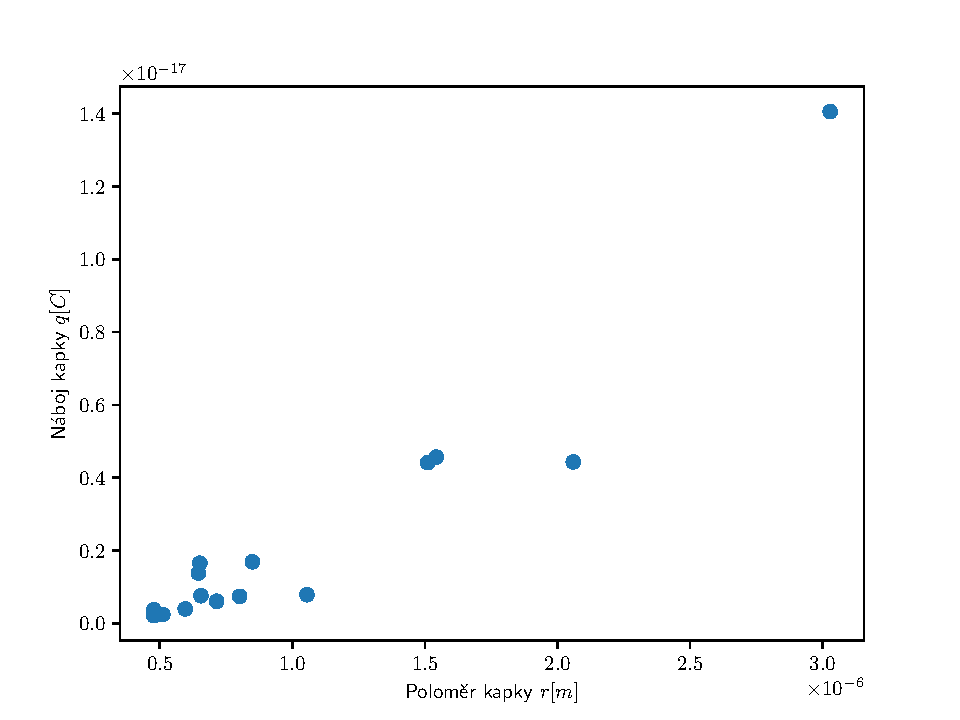
\includegraphics[scale=1]{data/graph1.pdf}
  \caption{Rutherfordův rozptyl}
\end{figure}
\begin{figure}[h]
  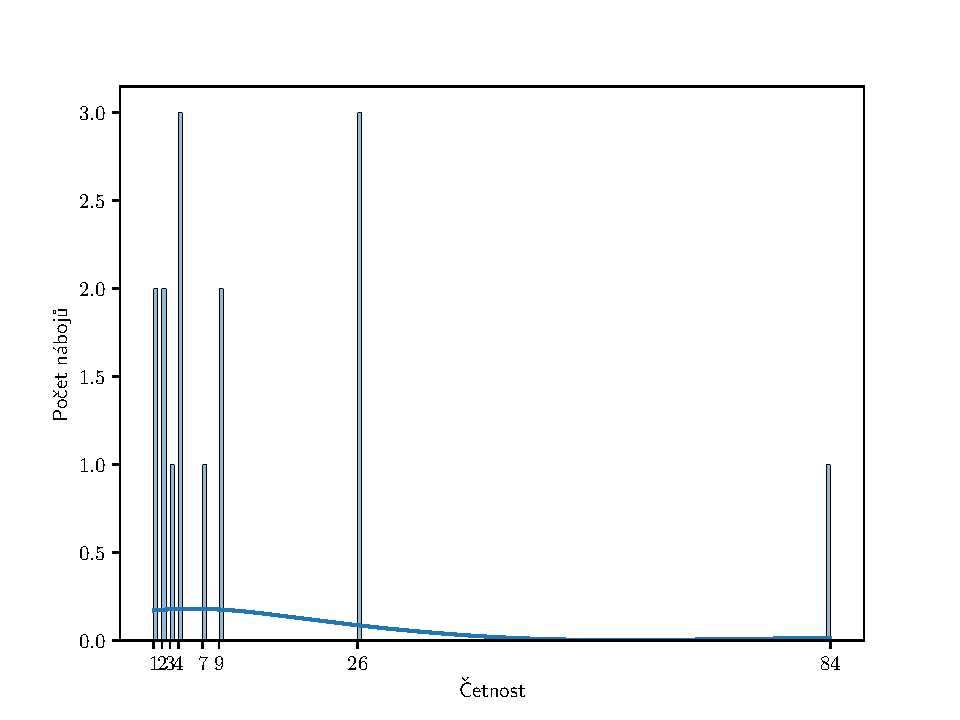
\includegraphics[scale=1]{data/hist.pdf}
  \caption{Rutherfordův rozptyl}
\end{figure}
\end{document}
